\documentclass[11pt]{article}
\usepackage{titling}
\usepackage[english]{babel}
\usepackage[margin=0.6in]{geometry} % Page Dimension
\usepackage{physoly}

%%%%%%%%%%%%%%%%%%%%%%%%%%%%%%%%%%%%%%%%%%
%                PACKAGES                %  
%%%%%%%%%%%%%%%%%%%%%%%%%%%%%%%%%%%%%%%%%%

% Styling Choices
\setlength{\parskip}{\baselineskip}%

% Math
\usepackage{amsmath, amsthm, amssymb}
\usepackage[inline]{asymptote}
\usepackage{xcolor}
\usepackage{cancel}

% Allows for hyperlinking
\usepackage{hyperref}
\hypersetup{
    colorlinks=true,
    linkcolor=magenta,
}

% Blind Footnote
\newcommand\blfootnote[1]{%
  \makeatletter{\footnotetext{#1}\makeatother}
}

% Fancy Header
\usepackage{fancyhdr}
\pagestyle{fancy}
\lhead{Kalda Mechanics}
\rhead{\thepage}

% Coloured Boxes
\usepackage{xcolor}
\definecolor{border}{HTML}{004D4D}
\definecolor{hard}{HTML}{ffccb3}
\definecolor{easy}{HTML}{b3e6b3}
\definecolor{normal}{HTML}{f2f2f2}

% Syntax: \colorboxed[<color model>]{<color specification>}{<math formula>}
\newcommand*{\colorboxed}{}
\def\colorboxed#1#{%
  \colorboxedAux{#1}%
}
\newcommand*{\colorboxedAux}[3]{%
  % #1: optional argument for color model
  % #2: color specification
  % #3: formula
  \begingroup
    \colorlet{cb@saved}{.}%
    \color#1{#2}%
    \boxed{%
      \color{cb@saved}%
      #3%
    }%
  \endgroup
}

% Setup Gray Solution Boxes
\usepackage[breakable,many]{tcolorbox}
\newtcolorbox[auto counter]{solution}[1]{
    enhanced, breakable,
    arc=0pt,
    % colback=default, % Background color
    colframe=white, % Border Color
    coltitle=black, % Title Color
    fonttitle=\bfseries,
    title=\fcolorbox{border}{#1}{\textcolor{border}{pr} \bfseries \textcolor{border}{\thetcbcounter}.},
    attach title to upper,
    after title={\ },
    segmentation style={dashed, gray},
}

% Title and front page
\title{Solutions to Problems in Mechanics Handout by Jaan Kalda With detailed diagrams and walkthroughs}
% Author
\author{\textsc{Ashmit Dutta, QiLin Xue, Kushal Thaman, Arhaan Ahmad}}

\begin{document}
\begin{titlepage}
    \begin{center}
        \vspace*{1cm}
 
        \Huge
        \textbf{Solutions to Jaan Kalda's Problems in Waves and Optics}
 
        \vspace{0.5cm}
        \LARGE
        \textbf{With detailed diagrams and walkthroughs}
        
        \vspace{0.1cm}
        Edition 1.3.1
        
        \vspace{1.2cm}
 
          Rakshit, Ashmit Dutta, Aarush Gupta,  Kushal Thaman, QiLin Xue, \\Daniel Yang
        \vspace{10mm}
\begin{center}
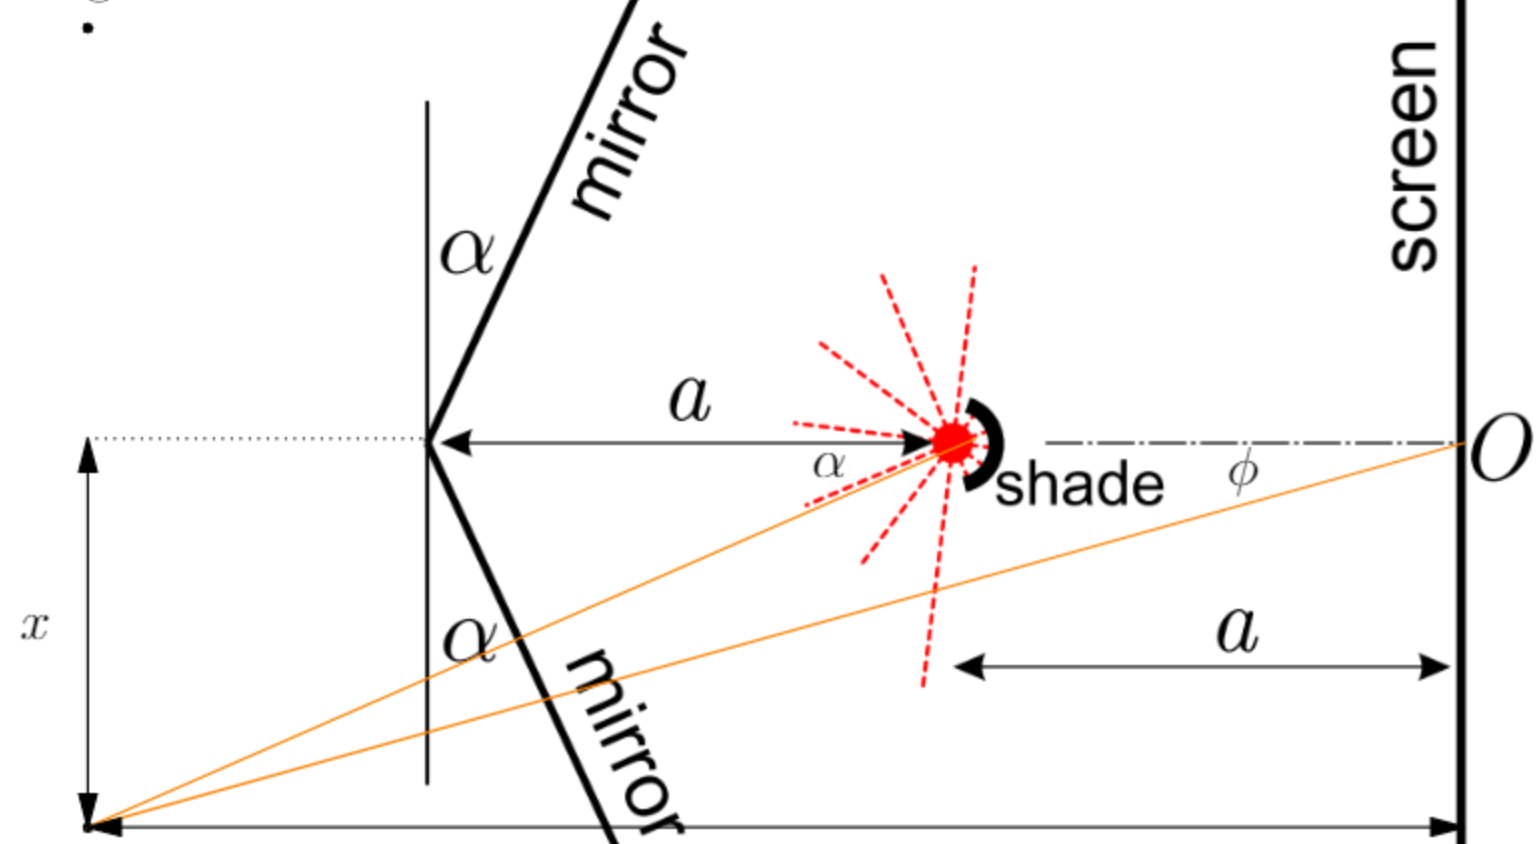
\includegraphics[width=15cm]{title.png}
\end{center}
        \vfill
        
        \Large
        Updated
        \today
 
    \end{center}
\end{titlepage}
\newpage
%%%%%%%%%%%
% Preface %
%%%%%%%%%%%
\section*{Preface}
\vspace{-5mm}
\indent Jaan Kalda's \href{https://www.ioc.ee/~kalda/ipho/}{handouts} are beloved by physics students both in for a quick challenge, to students preparing for international Olympiads. As of writing, the current \href{https://www.ioc.ee/~kalda/ipho/waveopt.pdf}{waves and optics} handout has 19 unique problems and 2 main `ideas'. \textbf{Many of the problems had solutions at the back of the handout. This solutions manual attempts to solve the problems that don't have solutions}.

This solutions manual came as a pilot project from the online community at \url{artofproblemsolving.com}. Although there were detailed hints provided, full solutions have never been written. The majority of the solutions seen here were written on a private forum given to those who wanted to participate in making solutions. In an amazing show of an online collaboration, students from around the world came together to discuss ideas and methods and created what we see today.

\subsection*{Structure of The Solutions Manual}
\vspace{-5mm}
Each chapter in this solutions manual will be directed towards a section given in Kalda's mechanics handout. There are three major chapters: statics, dynamics, and revision problems. If you are stuck on a problem, cannot make progress even with the hint, and come here for reference, look at only the start of the solution, then try again. Looking at the entire solution wastes the problem for you and ruins an opportunity for yourself to improve.

\subsection*{Contact Us}
\vspace{-5mm}
Despite editing, there is almost zero probability that there are \textit{no} mistakes inside this book. If there are any mistakes, you want to add a remark, have a unique solution, or know the source of a specific problem, then please contact us at \url{hello@physoly.tech}. The most current and updated version can be found on our website \url{physoly.tech}

Please feel free to contact us at the same email if you are confused on a solution. Chances are that many others will have the same question as you.

\newpage
\section{Solutions to Unsolved Problems Problems}
\vspace{-5mm}
This section will consist of the solutions to unsolved problems which do not have solutions at the back of the handout. These consist of problems 2, 3, 9, 15, 16, 17, 18, and 19. These problems vary from easy high school to hard physics olympiad problems.

\begin{solution}{normal}
The ice melts when the temperature of the kettle begins to drop. All the heat that was supplied to the kettle was used in melting the ice and bringing it up to the temperature of the rest of the water. Meanwhile the water already present lost some heat to the surroundings, and thus the graph dips at that point.
\vspace{3mm}

The total time for the temperature to recover to $T = 75^{\circ}\;\mathrm{C}$ is approximately $t = 37\;\mathrm{s}$. The heating rate of water is the slope of the graph or $dT/dt$. This means that the power at $T = 70^{\circ}\;\mathrm{C}$ is $P' = P \tan 75^{\circ}\approx 500\;\mathrm{W}$. Therefore, from energy conservation, we have that 
\[mL + mc\Delta T = Pt\implies m = \frac{Pt}{L + c\Delta T} \approx \boxed{28\;\mathrm{g}}.\]
\end{solution}
\begin{custom-simple}[Problem 3]
If the light is coherent, then the amplitude of the light emerging from each slit can individually be written as:
$$E=E_0\cos(\omega t + \phi)$$
where $\omega$ is the frequency and $\phi$ is the phase shift. An alternative way of writing this is:
$$E=E_0e^{i\omega t}e^{i\phi}$$
Its real component corresponds with the magnitude of the field that we measure at a certain time $t$. The complex number $e^{i\omega t}e^{i\phi}$ can be represented as a phasor which is essentially a vector with a constant magnitude of one that rotates in the complex plane at an angular frequency of $\omega$ (that is, it makes an angle $\omega t+\phi$ with the real axis). We want the sum of the three different amplitudes to sum up to zero, or:
$$E_1+E_2+E_3=E_0\cdot \left[e^{i\omega t}e^{i\phi_1}+e^{i\omega t}e^{i\phi_2}+e^{i\omega t}e^{i\phi_3}\right] = 0$$
Although this may look complicated, we can simplify it by treating them geometrically as phasors. To achieve an intensity minima of zero, we need three phasors such that their vector sum equals zero, which is equivalent to making a closed shape. Since they have the same magnitude, this shape must be an equilateral triangle. Without loss of generality, let $\phi_1=0$. This means $\phi_2=\phi_3=2\pi k + \frac{2\pi}{3}$ where $k$ is an integer.

The phase shift is defined as:
$$\frac{\phi}{2\pi} = \frac{(\text{path difference})}{\lambda} \implies k+ \frac{1}{3} = \frac{d\sin\theta}{\lambda}$$
where $d$ is the separation between two arbitrary slits and $\theta$ is the angle the light makes with the horizontal. Applying this for the slit separation distances in this problem, we have:
$$a = \left(k_1+\frac{1}{3}\right)\frac{\lambda}{\sin\theta_1}$$
$$b = \left(k_2+\frac{1}{3}\right)\frac{\lambda}{\sin\theta_2}$$
If we assume that $a,b \ll L$ where $L$ is the distance between the slits and the screen, then $\sin\theta_1=\sin\theta_2$. Taking the ratio, we get:
$$\frac{a}{b} = \frac{n}{m} \equiv \frac{3k_1+1}{3k_2+1}$$
This produces a minima of zero for any integer combinations of $k_1$ and $k_2$. We will prove that for each combination, $n-m$ is a multiple of three. We have:
$$3k_2+1 - (3k_2+1) = 3r \implies 3(k_2-k_1)=3r \implies k_2-k_1=r$$
where $r$ is an integer. Since $k_1$ and $k_2$ have to be integers, then $r$ must also be an integer, proving the statement.
\end{custom-simple}
\begin{solution}{normal}
Let us assume that $-dm'$ mass sublimes at some instant. ($m'$ is the total mass of the cup.)
Intially it is moving with $v$, the velocity of the vessel
Finally its velocity \textit{with respect to the vessel}, in the \textit{direction of motion} of the vessel becomes $-\frac{\sqrt {\frac{3RT}{\mu}}}{\sqrt 3}=-\sqrt{\frac{RT}{\mu}}.$\footnote{Since the rms speed is randomly directed in $x, y, z$ directions and we only want one speed, we divide by the magnitude of the unit vectors.}
Thus, it provides an impulse, $-(-dm' \Delta v )= -dm'\sqrt{\frac{RT}{\mu}}$ to the vessel
$$\therefore v = \int dv=\int_{M+m}^{M}\frac{-dm'\sqrt{\frac{RT}{\mu}}}{m'}=\sqrt{\frac{RT}{\mu}}\textup{ln}\left (1+\frac{m}{M}  \right )\approx \boxed{\sqrt{\frac{RT}{\mu}}\frac{m}{M}} $$
\end{solution}
\begin{solution}{normal}
Due to symmetry the turtles meet at the centroid of the triangle formed, and form an equilateral triangle at any instant. The velocity of the first turtle with respect to the other is obviously $$0.1 \cos\left(60\degree\right) \;\text{m/s}$$

Thus, the relative velocity of separation is
$$v(1+\cos\left(60\degree\right)) = \frac{3v}{2}$$

Since this is constant, the time taken for the turtles to meet is
$$t = \frac{d}{\tfrac{3v}{2}} = \frac{2d}{3v} = \boxed{6.7\;\text{s}}$$

\tcbline

\textbf{Solution 2:} The path length of any turtle in the motion is simply
$$ds = dr\sqrt{1+\left(\frac{rd\theta}{dr}^2\right)}$$

Using polar coordinates, one can deduce that
\begin{align*}
\frac{dr}{dt} &= -10\sin\left(60\degree\right)\\
v\frac{d\theta}{dt} &= \frac{10}{2}=5
\end{align*}

Hence we have
$$\frac{d\theta}{dr} = -\frac{1}{r\sqrt{3}} \Rightarrow ds = \frac{2dr}{\sqrt{3}}$$

Since $t = \dfrac{ds}{10} $, we find the total time by integrating this expression:
\begin{align*}
\int_{0}^{T}{dt} &= -\frac{2}{\sqrt{3}v}\int_{\frac{1}{\sqrt{3}}}^{0}{dr}\\
T &=  \frac{2d}{3v} = \boxed{6.7\;\text{s}}
\end{align*}
\end{solution}
\begin{custom-simple}[Problem 16]
\begin{enumerate}
\item There is no light coming out from outlet $C_2$ because at the junction point a wave is generated in upper fiber in the same direction as the circular fiber (Huygens principle can be used to prove this).As energy at steady state is constant we can say that the total energy input $=$ total energy output, hence $I_{A_2}+I_{C_1}=I_0$. The result is a mirror image of the graph in the problem text that touches $I = 0$ at the bottom and $I = I_0$ at the top.
\item At this wavelength, all intensity $I_0$ comes out from fiber $C_1$ and intensity in fiber $B$ and intensity in direction $C_1$ should have ratio $(1-\alpha)/\alpha$. So $$I_B = \frac{I_0(1-\alpha)}{\alpha} = 99I_0$$
\item The intensity of light in fiber B is maximum when the light circulating in the fiber reaches the lower junction point in the same phase as the light from fiber A. Then the intensity going to fiber C is also maximum. Thus, fiber B must accommodate an integer of n wavelengths. From the graph we see that two successive resonances occur at wavelengths $\lambda_0 = 1660$ nm and $\lambda_1 = 1680$ nm. So $n\lambda_1 ’ = (n+1) \lambda_0 ’= l$, where $l$ is the desired length and the second resonant wavelength in the fiber is $\lambda_1 ’ = \lambda_0 ’\frac{\lambda_1 }{\lambda_0}$. From this relation we find $\frac{1}{n}= \frac{\lambda_1 ’}{\lambda_0 ’} - 1$ and
$$ l = \frac {\lambda_0 ’\lambda_1}{\lambda_1-\lambda_0} = \boxed{84\;\mathrm{\mu m}}$$
\end{enumerate}
\end{custom-simple}
\newpage
\begin{solution}{normal}
From the prelude, we have the work as:
$$W = \frac{m}{2}(v_2^2-v_1^2) + \Delta U$$
The internal energy changes both in gravitational energy and in internal energy so:
\begin{align*}
\Delta U &= mg\Delta h + nC_v\Delta T \\
&= mg\Delta h + \left(nR\Delta T\right)\frac{C_v}{R} \\
&= mg\Delta h + \Delta(PV)\frac{C_v}{R} \\
\end{align*}
The compression work $W$ is:
$$W=-\Delta(PV)$$
so putting everything together gives:
$$0=\frac{m}{2}(v_2^2-v_1^2)+mg\Delta h + \Delta(PV) \left(\frac{C_v+R}{R}\right)$$
Having $C_P=C_V+R$, $\Delta(PV)=nR\Delta T$, and letting the molar mass $\mu\equiv m/n$, we can simplify this to: 
$$0=\frac{1}{2}(v_2^2-v_1^2)+g(h_2-h_1) + \frac{C_P(T_2-T_1)}{\mu}\implies \frac{1}{2}v^2 + gh + c_p T = 0$$
\end{solution}
\begin{custom-simple}[Problem 18]
\textbf{(a)} By energy conservation, the amplitudes of the output wave and input wave must be the same. The output fiber wave is formed by the sum of the wave in the fiber and the wave from the other fiber. According to the energy conservation, the amplitude of each component is $\sqrt 2$ times smaller than the original when the wave enters only one fiber. Thus, while the amplitude of the incoming waves was A, the outgoing resultant wave is in an expressible form.
$$A = \sqrt {\left(\frac {A}{\sqrt 2}\right)^2 \cdot 2 + 2\left(\frac {A}{\sqrt 2}\right) \left(\frac {A}{\sqrt 2}\right)\cos \phi}$$where $\phi$ is the phase shift. So $\cos (\phi/ 2) = 1/\sqrt 2$ and consequently $\phi = \frac {\pi}{2}$
\vspace{5mm}

\textbf{(b)} Phase difference between the $2$ fibers is $\pi$, the minima condition in fiber $1$ is $\Delta l = n\lambda$, where n is an integer. Writing this as $n = \frac{\Delta l}{\lambda}$ we see that
\[\frac{\Delta l}{\lambda_{\text{min}}}\geq n \geq \frac{\Delta l}{\lambda_{\text{max}}}\]thus $49.2 \geq n \geq 45.4$ and the values of $n$ to be sought are $46, 47, 48$ and $49$. The corresponding wavelengths are given by the formula $\lambda = \frac{n}{\Delta l}$; these are $612, 625, 638$ and $652\;\mathrm{nm}$
\end{custom-simple}
\begin{solution}{normal}
Consider a horizontal displacement of a gas. The impulse the gas experiences is:
$$J = F_\text{net} dt = \Delta p S dt = (p_1-p_2)Sdt$$
where $S$ is the cross sectional area. Take $p_1 > p_2$ such that the gas is moving towards the right (which we arbitrarily set as the positive direction). This gives the change in momentum to be:
$$\Delta p =(\rho Sx_2)v_2-(\rho Sx_1)v_1 =(\rho S)v_2^2 dt-(\rho Sx_1)v_1^2 dt$$
Setting these two expressions equal gives:
$$p_1-p_2=\rho v_2^2 - \rho v_1^2$$
Since this is true for any two intervals, then the quantity
$$p+\rho v^2 = \text{constant}$$
must be preserved.
\end{solution}

\end{document}